\section{changePassword(String oldPassword, String newPassword, String confirmPassword)}

Il metodo \colorbox{lightgray}{changePassword}, appartenente alla classe \colorbox{lightgray}{AuthService}, è responsabile della modifica della password di un utente. Per la sua particolare struttura, si è scelto di adottare una \textbf{strategia di testing white-box}, poiché il metodo è costituito principalmente da \textbf{controlli logici} e di contesto, come la verifica della correttezza della vecchia password e la conformità della nuova password al pattern richiesto.
\\
Di seguito è riportato il \textbf{Grafo del Flusso di Controllo del metodo}, seguito dai \textbf{test case} sviluppati per garantire la copertura di \textbf{tutti i cammini possibili} all’interno del grafo.

\begin{figure}[H]
	\centering
	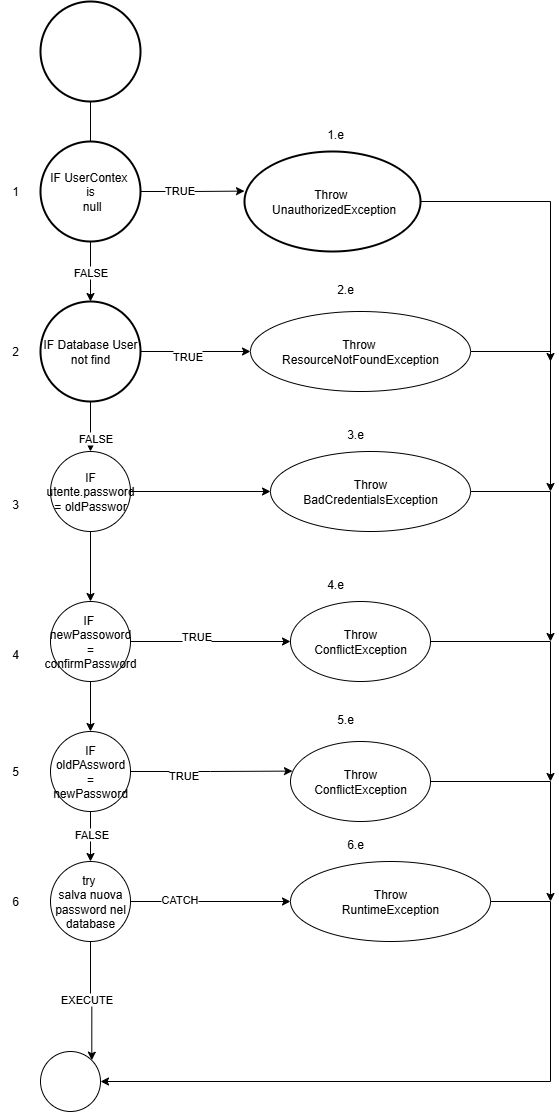
\includegraphics[width=0.7\linewidth]{Immagini/unit test/grafoCambiaPassword.png}
	\caption[GFC changePassword]{GFC del metodo changePassword(String oldPassword, String newPassword, String confirmPassword)}
\end{figure}

% Configurazione listings
\lstset{
	language=Java,                % Linguaggio di esempio
	backgroundcolor=\color{bgcolor}, % Colore di sfondo
	basicstyle=\ttfamily\small,     % Font e dimensione
	keywordstyle=\color{keywordcolor}\bfseries,
	commentstyle=\color{commentcolor}\itshape,
	stringstyle=\color{stringcolor},
	numbers=left,                   % Numeri a sinistra
	numberstyle=\tiny\color{gray},  % Stile dei numeri
	stepnumber=1,                   % Numeri in ogni riga
	numbersep=5pt,                  % Distanza dai numeri
	frame=single,                   % Cornice intorno al codice
	rulecolor=\color{gray},         % Colore della cornice
	tabsize=4,                       % Tab = 4 spazi
	showstringspaces=false,
	breaklines=true,                  % A capo automatico se troppo lungo
	literate=
	{à}{{\`a}}1
	{è}{{\`e}}1
	{é}{{\'e}}1
	{ì}{{\`i}}1
	{ò}{{\`o}}1
	{ù}{{\`u}}1
}


\begin{lstlisting}
	 /**
	*  Questo test copre i nodi da 1 al 6 percorrendo solo il cammino senza errori.
	*/
	@Test
	void changePassword_ShouldSave_WhenValid() {
		User mockUser = new User();
		mockUser.setId(1);
		
		mockUser.setPassword(passwordEncoder.encode("oldPass"));
		
		
		mocked.when(UserContex::getUserCurrent).thenReturn(mockUser);
		
		when(userRepository.findById(1)).thenReturn(Optional.of(mockUser));
		
		String result = authService.changePassword("oldPass", "newPass", "newPass");
		
		verify(userRepository).save(mockUser);
		assertEquals(Msg.PASSWORD_CHANGED, result);
		//assert true when password encorder match new password with mockUser password
		assertTrue(passwordEncoder.matches("newPass", mockUser.getPassword()));
		
	}
\end{lstlisting}

\begin{lstlisting}
	/**
	* Questo test copre il nodo 1 e 1.e
	* * verifica che venga lanciata una UnauthorizedException quando l'utente non viene trovato nel userContex.
	*/
	@Test
	void changePassword_
	ShouldThrowUnauthorizedException_WhenUserContextNotFound() {
		
		mocked.when(UserContex::getUserCurrent).thenReturn(null);
		Exception ex = assertThrows(it.unina.dietiestates25.exception.UnauthorizedException.class, () ->authService.changePassword("oldPass", "newPass", "newPass") );
	}
\end{lstlisting}
	
\begin{lstlisting}
	/**
	* Questo test copre i nodi 1, 2, 2.e
	* * verifica che venga lanciata una ResourceNotFoundException quando l'utente non viene trovato nel database.
	*/
	@Test
	void changePassword_
	ShouldThrowResourceNotFoundException_WhenUserNotFoundInDB() {
		
		User mockUser = new User();
		mockUser.setId(1);
		
		
		mocked.when(UserContex::getUserCurrent).thenReturn(mockUser);
		
		when(userRepository.findById(1)).thenReturn(Optional.empty());
		
		assertThrows(it.unina.dietiestates25.exception.ResourceNotFoundException.class, () ->authService.changePassword("oldPass", "newPass", "newPass") );
		
	}
\end{lstlisting}
	
\begin{lstlisting}
	/**
	* Questo test copre i nodi 1, 2, 3, 3.e
	* * verifica che venga lanciata una BadCredentialsException quando la vecchia password non corrisponde alla password corrente del user.
	*/
	@Test
	void changePassword_
	ShouldThrowBadCredentialsException_WhenOldPasswordNotMatch() {
		User mockUser = new User();
		mockUser.setId(1);
		mockUser.setPassword(passwordEncoder.encode("oldPass"));
		
		mocked.when(UserContex::getUserCurrent).thenReturn(mockUser);
		
		when(userRepository.findById(1)).thenReturn(Optional.of(mockUser));
		
		assertThrows(BadCredentialsException.class, () ->authService.changePassword("wrongOldPass", "newPass", "newPass") );
	}
\end{lstlisting}

\begin{lstlisting}
	/**
	* Questo test copre i nodi 1, 2, 3, 4, 4.e
	* * verifica che venga lanciata una ConflictException quando la nuova password e la password di conferma non corrispondono.
	*/
	@Test
	void changePassword_ShouldThrowConflictException
	_WhenNewPasswordNotMatchConfirmPassword() {
		
		User mockUser = new User();
		mockUser.setId(1);
		mockUser.setPassword(passwordEncoder.encode("oldPass"));
		
		mocked.when(UserContex::getUserCurrent).thenReturn(mockUser);
		
		when(userRepository.findById(1)).thenReturn(Optional.of(mockUser));
		
		assertThrows(it.unina.dietiestates25.exception.ConflictException.class, () ->authService.changePassword("oldPass", "newPass", "differentNewPass") );
	}
\end{lstlisting}

\begin{lstlisting}
	 /**
	* Questo test copre i nodi 1, 2, 3, 4, 5, 5.e
	* * verifica che venga lanciata una ConflictException quando la nuova password è uguale alla password attuale.
	*/
	@Test
	void changePassword_ShouldThrowConflictException
	_WhenNewPasswordIsSameAsOldPassword() {
		User mockUser = new User();
		mockUser.setId(1);
		mockUser.setPassword(passwordEncoder.encode("oldPass"));
		
		mocked.when(UserContex::getUserCurrent).thenReturn(mockUser);
		
		when(userRepository.findById(1)).thenReturn(Optional.of(mockUser));
		
		assertThrows(it.unina.dietiestates25.exception.ConflictException.class, () ->authService.changePassword("oldPass", "oldPass", "oldPass") );
	}
\end{lstlisting}

\begin{lstlisting}
	/**
	* Questo test copre i nodi 1, 2, 3, 4, 5, 6, 6.e
	* * verifica che venga lanciata una RuntimeException quando si verifica un errore durante il salvataggio della nuova password.
	*/
	@Test
	void changePassword_ShouldThrowRuntimeException_WhenErrorOnSave() {
		User mockUser = new User();
		
		mockUser.setId(1);
		mockUser.setPassword(passwordEncoder.encode("oldPass"));
		
		
		mocked.when(UserContex::getUserCurrent).thenReturn(mockUser);
		
		when(userRepository.findById(1)).thenReturn(Optional.of(mockUser));
		//simula un errore durante il salvataggio
		when(userRepository.save(mockUser)).thenThrow(new RuntimeException());
		
		assertThrows(RuntimeException.class, () ->authService.changePassword("oldPass", "newPass", "newPass") );
	}
\end{lstlisting}

\begin{figure}[H]
	\centering
	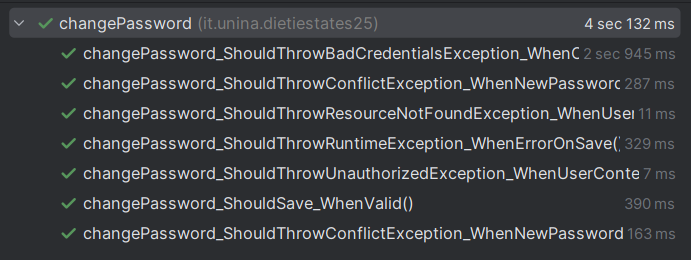
\includegraphics[width=0.7\linewidth]{Immagini/unit test/esitiTestChangePassword.png}
	\caption[Esito test 4]{Screen che riporta l'esito positivo dei test}
\end{figure}
